\documentclass{article}
\usepackage{tikz}
\usepackage{amsmath}
\begin{document}
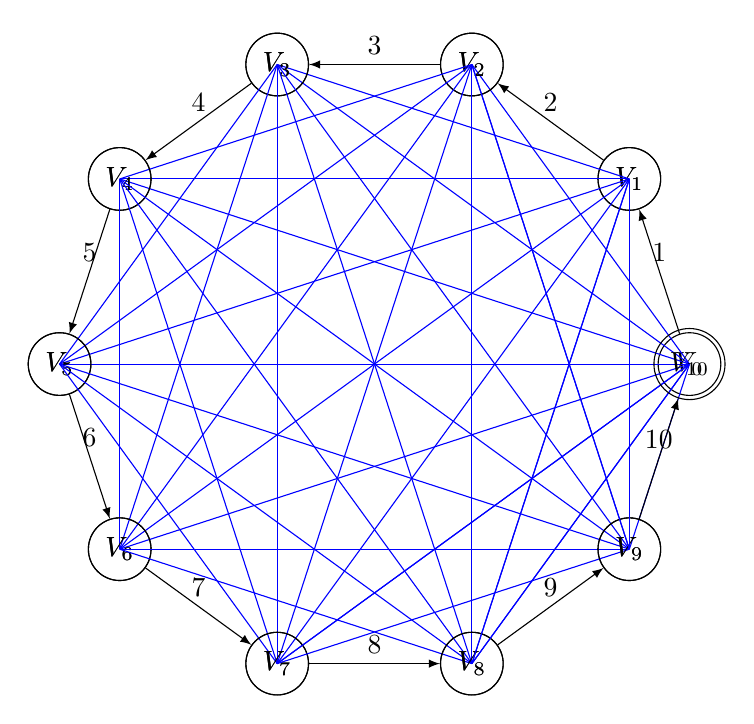
\begin{tikzpicture}[scale = 0.5]
	\pgfmathsetmacro {\n}{10};
	\pgfmathsetmacro{\p}{360/\n};
	\pgfmathsetmacro{\e}{360-\p};
    \foreach \x in {0,\p,...,\e} {
		\pgfmathsetmacro{\a}{int(round((\x + \p)/\p))};
		\newcounter{mycounter\a}
		\setcounter{mycounter\a}{\x + \p}
		\ifnum \value{mycounter\a} < 181 {
			\ifnum \value{mycounter\a} < 45
			\node[shape=circle,draw=black] (\a+1) at (\x:8cm) {$V_{\the\numexpr\a - 1 \relax}$};
			\node[shape=circle,draw=black] (\a+2) at (\x+ \p:8cm) {$V_{\a}$};
			\path[-latex]
			(\a+1)  edge node[above] {$\a$} (\a+2); 
			 %(\x+ \p:8cm) node [at start,right] {$V_{\a}$};
			\else
				\ifnum \value{mycounter\a} < 135
				\node[shape=circle,draw=black] (\a+2) at (\x:8cm) {$V_{\the\numexpr\a - 1 \relax}$};
				\node[shape=circle,draw=black] (\a+3) at (\x+ \p:8cm) {$V_{\a}$};
			\path[-latex]
			
				
				(\a+2) edge node[above] {$\a$} (\a+3);
				\else
				\node[shape=circle,draw=black] (\a+3) at (\x:8cm) {$V_{\the\numexpr\a - 1 \relax}$};
				\node[shape=circle,draw=black] (\a+4) at (\x+ \p:8cm) {$V_{\a}$};
			\path[-latex]
			
				
				(\a+3) edge node[above] {$\a$} (\a+4);
				\fi
			\fi
		}
		\else {
			\ifnum \value{mycounter\a} < 225
			\node[shape=circle,draw=black] (\a+4) at (\x:8cm) {$V_{\the\numexpr\a - 1 \relax}$};
			\node[shape=circle,draw=black] (\a+5) at (\x+ \p:8cm) {$V_{\a}$};
			\path[-latex]
			
				
				(\a+4) edge node[above] {$\a$} (\a+5);
			\else
				\ifnum \value{mycounter\a} < 315
				\node[shape=circle,draw=black] (\a+5) at (\x:8cm) {$V_{\the\numexpr\a - 1 \relax}$};
				\node[shape=circle,draw=black] (\a+6) at (\x+ \p:8cm) {$V_{\a}$};
			\path[-latex]
			
				
				(\a+5) edge node[above] {$\a$} (\a+6);
				\else
					\node[shape=circle,draw=black] (\a+6) at (\x:8cm) {$V_{\the\numexpr\a - 1 \relax}$};
````				\node[shape=circle,draw=black] (\a+7) at (\x+ \p:8cm) {$V_{\a}$};
			\path[-latex]
			
				
				(\a+6) edge node[above] {$\a$} (\a+7);
				\fi
			\fi
		}
		\fi
		\pgfmathsetmacro{\d}{\x + 2*\p};
		\pgfmathsetmacro{\n}{\x + 3*\p};
		\foreach \y in {\d,\n,...,\e} {
   			\draw[blue] (\x:8cm) -- (\y:8cm);
		}
	}
\end{tikzpicture}
\end{document}
